
\documentclass[letterpaper,hide notes,xcolor={table,svgnames},pdftex,10pt]{beamer}
\def\showexamples{t}

\usecolortheme{crane}
\setbeamertemplate{navigation symbols}{}

\usetheme{MyPittsburgh}
\usepackage{hyperref}
\usepackage{graphicx,xspace}
\usepackage[normalem]{ulem}
\usepackage{multicol}
\usepackage{amsmath,amssymb,amsthm,graphicx,xspace}
\newcommand\SF[1]{$\bigstar$\footnote{SF: #1}}

\usepackage[sfdefault,lf]{carlito}
\usepackage[T1]{fontenc}
\usepackage[scaled]{beramono}
\usepackage{tikzpagenodes}
\newcommand{\Rplus}{\protect\hspace{-.1em}\protect\raisebox{.35ex}{\small{\small\textbf{+}}}}
\newcommand{\Cpp}{\mbox{C\Rplus\Rplus}\xspace}

\newcounter{tmpnumSlide}
\newcounter{tmpnumNote}

\newcommand\mnote[1]{%
	\addtocounter{tmpnumSlide}{1}
	\ifdefined\showcues {~\tiny\fbox{\arabic{tmpnumSlide}}}\fi
	\note{\setlength{\parskip}{1ex}\addtocounter{tmpnumNote}{1}\textbf{\Large \arabic{tmpnumNote}:} {#1\par}}}

\newcommand\mmnote[1]{\note{\setlength{\parskip}{1ex}#1\par}}


\newcommand\mquestion[2]{{~\color{red}\fbox{?}}\note{\setlength{\parskip}{1ex}\par{\Large \textbf{?}} #1} \note{\setlength{\parskip}{1ex}\par{\Large \textbf{A}} #2\par}\ifdefined \presentationonly \pause \fi}

\newcommand\blackboard[1]{%
	\ifdefined   \showblackboard
		{#1}
	\else {\begin{center} \fbox{\colorbox{blue!30}{%
						\begin{minipage}{.95\linewidth}%
							\hspace{\stretch{1}} Some space intentionally left blank; done at the blackboard.%
						\end{minipage}}}\end{center}}%
	\fi%
}

\usepackage{listings}
\lstset{%
	keywordstyle=\bfseries,
	aboveskip=15pt,
	belowskip=15pt,
	captionpos=b,
	identifierstyle=\ttfamily,
	frame=lines,
	numbers=left, basicstyle=\scriptsize, numberstyle=\tiny, stepnumber=0, numbersep=2pt}

\usepackage{siunitx}
\newcommand\sius[1]{\num[group-separator = {,}]{#1}\si{\micro\second}}
\newcommand\sims[1]{\num[group-separator = {,}]{#1}\si{\milli\second}}
\newcommand\sins[1]{\num[group-separator = {,}]{#1}\si{\nano\second}}
\sisetup{group-separator = {,}, group-digits = true}

%% -------------------- tikz --------------------
\usepackage{tikz}
\usetikzlibrary{positioning}
\usetikzlibrary{arrows,backgrounds,automata,decorations.shapes,decorations.pathmorphing,decorations.markings,decorations.text}

\tikzstyle{place}=[circle,draw=blue!50,fill=blue!20,thick, inner sep=0pt,minimum size=6mm]
\tikzstyle{transition}=[rectangle,draw=black!50,fill=black!20,thick, inner sep=0pt,minimum size=4mm]

\tikzstyle{block}=[rectangle,draw=black, thick, inner sep=5pt]
\tikzstyle{bullet}=[circle,draw=black, fill=black, thin, inner sep=2pt]

\tikzstyle{pre}=[<-,shorten <=1pt,>=stealth',semithick]
\tikzstyle{post}=[->,shorten >=1pt,>=stealth',semithick]
\tikzstyle{bi}=[<->,shorten >=1pt,shorten <=1pt, >=stealth',semithick]

\tikzstyle{mut}=[-,>=stealth',semithick]

\tikzstyle{treereset}=[dashed,->, shorten >=1pt,>=stealth',thin]

\usepackage{ifmtarg}
\usepackage{xifthen}
\makeatletter
% new counter to now which frame it is within the sequence
\newcounter{multiframecounter}
% initialize buffer for previously used frame title
\gdef\lastframetitle{\textit{undefined}}
% new environment for a multi-frame
\newenvironment{multiframe}[1][]{%
	\ifthenelse{\isempty{#1}}{%
		% if no frame title was set via optional parameter,
		% only increase sequence counter by 1
		\addtocounter{multiframecounter}{1}%
	}{%
		% new frame title has been provided, thus
		% reset sequence counter to 1 and buffer frame title for later use
		\setcounter{multiframecounter}{1}%
		\gdef\lastframetitle{#1}%
	}%
	% start conventional frame environment and
	% automatically set frame title followed by sequence counter
	\begin{frame}%
		\frametitle{\lastframetitle~{\normalfont(\arabic{multiframecounter})}}%
		}{%
	\end{frame}%
}
\makeatother

\makeatletter
\newdimen\tu@tmpa%
\newdimen\ydiffl%
\newdimen\xdiffl%
\newcommand\ydiff[2]{%
	\coordinate (tmpnamea) at (#1);%
	\coordinate (tmpnameb) at (#2);%
	\pgfextracty{\tu@tmpa}{\pgfpointanchor{tmpnamea}{center}}%
	\pgfextracty{\ydiffl}{\pgfpointanchor{tmpnameb}{center}}%
	\advance\ydiffl by -\tu@tmpa%
}
\newcommand\xdiff[2]{%
	\coordinate (tmpnamea) at (#1);%
	\coordinate (tmpnameb) at (#2);%
	\pgfextractx{\tu@tmpa}{\pgfpointanchor{tmpnamea}{center}}%
	\pgfextractx{\xdiffl}{\pgfpointanchor{tmpnameb}{center}}%
	\advance\xdiffl by -\tu@tmpa%
}
\makeatother
\newcommand{\copyrightbox}[3][r]{%
	\begin{tikzpicture}%
		\node[inner sep=0pt,minimum size=2em](ciimage){#2};
		\usefont{OT1}{phv}{n}{n}\fontsize{4}{4}\selectfont
		\ydiff{ciimage.south}{ciimage.north}
		\xdiff{ciimage.west}{ciimage.east}
		\ifthenelse{\equal{#1}{r}}{%
			\node[inner sep=0pt,right=1ex of ciimage.south east,anchor=north west,rotate=90]%
			{\raggedleft\color{black!50}\parbox{\the\ydiffl}{\raggedright{}#3}};%
		}{%
			\ifthenelse{\equal{#1}{l}}{%
				\node[inner sep=0pt,right=1ex of ciimage.south west,anchor=south west,rotate=90]%
				{\raggedleft\color{black!50}\parbox{\the\ydiffl}{\raggedright{}#3}};%
			}{%
				\node[inner sep=0pt,below=1ex of ciimage.south west,anchor=north west]%
				{\raggedleft\color{black!50}\parbox{\the\xdiffl}{\raggedright{}#3}};%
			}
		}
	\end{tikzpicture}
}


%% --------------------

%\usepackage[excludeor]{everyhook}
%\PushPreHook{par}{\setbox0=\lastbox\llap{MUH}}\box0}

%\vspace*{\stretch{1}

%\setbox0=\lastbox \llap{\textbullet\enskip}\box0}

\setlength{\parskip}{\fill}

\newcommand\noskips{\setlength{\parskip}{1ex}}
\newcommand\doskips{\setlength{\parskip}{\fill}}

\newcommand\xx{\par\vspace*{\stretch{1}}\par}
\newcommand\xxs{\par\vspace*{2ex}\par}
\newcommand\tuple[1]{\langle #1 \rangle}
\newcommand\code[1]{{\sf \footnotesize #1}}
\newcommand\ex[1]{\uline{Example:} \ifdefined \presentationonly \pause \fi
	\ifdefined\showexamples#1\xspace\else{\uline{\hspace*{2cm}}}\fi}

\newcommand\ceil[1]{\lceil #1 \rceil}


\AtBeginSection[]
{
	\begin{frame}
		\frametitle{Outline}
		\tableofcontents[currentsection]
	\end{frame}
}



\pgfdeclarelayer{edgelayer}
\pgfdeclarelayer{nodelayer}
\pgfsetlayers{edgelayer,nodelayer,main}

\tikzstyle{none}=[inner sep=0pt]
\tikzstyle{rn}=[circle,fill=Red,draw=Black,line width=0.8 pt]
\tikzstyle{gn}=[circle,fill=Lime,draw=Black,line width=0.8 pt]
\tikzstyle{yn}=[circle,fill=Yellow,draw=Black,line width=0.8 pt]
\tikzstyle{empty}=[circle,fill=White,draw=Black]
\tikzstyle{bw} = [rectangle, draw, fill=blue!20,
text width=4em, text centered, rounded corners, minimum height=2em]

\newcommand{\CcNote}[1]{% longname
	This work is licensed under the \textit{Creative Commons #1 3.0 License}.%
}
\newcommand{\CcImageBy}[1]{%
	\includegraphics[scale=#1]{creative_commons/cc_by_30.pdf}%
}
\newcommand{\CcImageSa}[1]{%
	\includegraphics[scale=#1]{creative_commons/cc_sa_30.pdf}%
}
\newcommand{\CcImageNc}[1]{%
	\includegraphics[scale=#1]{creative_commons/cc_nc_30.pdf}%
}
\newcommand{\CcGroupBySa}[2]{% zoom, gap
	\CcImageBy{#1}\hspace*{#2}\CcImageNc{#1}\hspace*{#2}\CcImageSa{#1}%
}
\newcommand{\CcLongnameByNcSa}{Attribution-NonCommercial-ShareAlike}

\newenvironment{changemargin}[1]{% 
	\begin{list}{}{% 
		\setlength{\topsep}{0pt}% 
		\setlength{\leftmargin}{#1}% 
		\setlength{\rightmargin}{1em}
		\setlength{\listparindent}{\parindent}% 
		\setlength{\itemindent}{\parindent}% 
		      \setlength{\parsep}{\parskip}% 
		      }% 
		\item[]}{\end{list}}





\title{Lecture 12 --- Processes and Threads }

\author{Jeff Zarnett \\ \small \texttt{jzarnett@uwaterloo.ca}}
\institute{Department of Electrical and Computer Engineering \\
	University of Waterloo}
\date{\today}

\begin{document}

\begin{frame}
  \titlepage
\end{frame}

\begin{frame}
	\frametitle{Processes}


	Early computers did exactly one thing.

	Or at least, exactly one thing at a time.

	Now the OS supports multiple programs running concurrently.

	To manage this complexity, the OS uses the \alert{process}.

\end{frame}

\begin{frame}
	\frametitle{The Process}

	A process is a program in execution.

	\begin{enumerate}
		\item The instructions and data.
		\item The current state.
		\item Any resources that are needed to execute.
	\end{enumerate}

\end{frame}

\begin{frame}
	\frametitle{Process Control Block}

	Data structure for managing processes: \alert{Process Control Block} (PCB).

	It contains everything the OS needs to know about the program.

	It is created and updated by the OS for each running process.

	It can be thrown away when the program has finished executing and cleaned up.

	The blocks are held in memory and maintained in some container by the kernel.


\end{frame}

\begin{frame}
	\frametitle{Process Control Block}

	The process control block will (usually) have:
	\begin{itemize}
		\item \textbf{Identifier.}
		\item \textbf{State.}
		\item \textbf{Priority.}
		\item \textbf{Program Counter*.}
		\item \textbf{Register Data*.}
		\item \textbf{Memory Pointers.}
		\item \textbf{I/O Status Information.}
		\item \textbf{Accounting Information.}
	\end{itemize}

\end{frame}

\begin{frame}
	\frametitle{Process Control Block (Simplified)}

	\begin{center}
		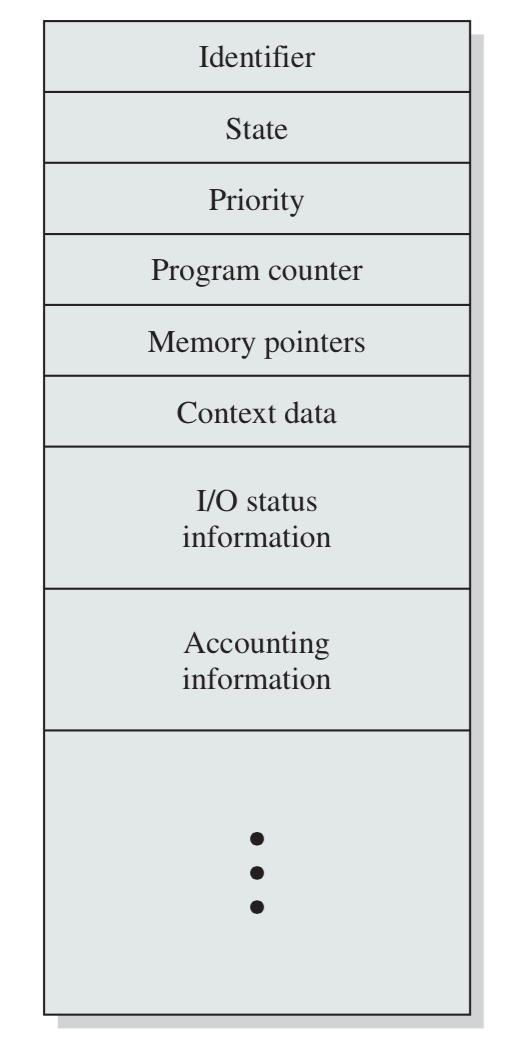
\includegraphics[width=0.35\textwidth]{images/pcb.png}
	\end{center}

\end{frame}

\begin{frame}
	\frametitle{The Circle of Life}


	Unlike energy, processes may be created and destroyed.

	Upon creation, the OS will create a new PCB for the process.\\
	\quad Also initialize the data in that block.
	
\end{frame}

\begin{frame}
	\frametitle{The Circle of Life}

	Set: variables to their initial values.\\
	\quad the initial program state.\\
	\quad the instruction pointer to the first instruction in \texttt{main}

	Add the PCB to the set.

	After the program is terminated and cleaned up:\\
	\quad Collect some data (like a summary of accounting information).\\
	\quad Remove the PCB from its list of active processes and carry on.


\end{frame}

\begin{frame}
	\frametitle{Process Creation}

	Three main events that may lead to the creation of a process:

	\begin{enumerate}
		\item System boot up.
		\item User request.
		\item One process spawns another.
	\end{enumerate}


\end{frame}

\begin{frame}
	\frametitle{Process Creation: At Boot Up}

	When the computer boots up, the OS starts and creates processes.

	An embedded system might have all the processes it will ever run.

	General-purpose operating systems: allow one (both) of the other ways.


\end{frame}

\begin{frame}
	\frametitle{Process Creation: At Boot Up}

	Some processes will be in the foreground; some in the background.

	A user-visible process: log in screen.

	Background process: server that shares media on the local network.

	UNIX term for a background process is \alert{Daemon}.

	Example: \texttt{ssh} (Secure Shell) command to log into a Linux system.


\end{frame}

\begin{frame}
	\frametitle{Process Creation: Users}

	Users are well known for starting up processes whenever they feel like it.\\
	\quad Much to the chagrin of system designers everywhere.

	Every time you double-click an icon or enter a command line command (like \texttt{ssh} above) that will result in the creation of a process.


	\begin{center}
		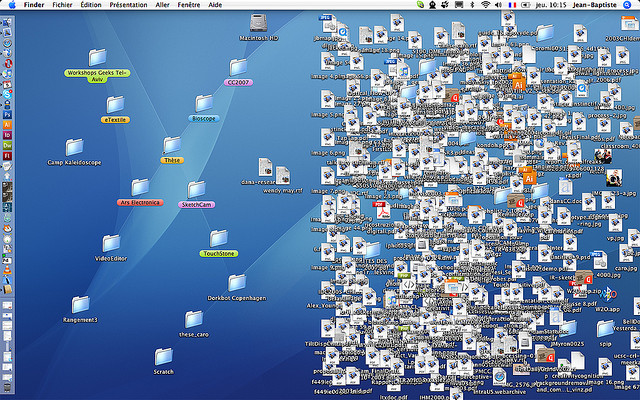
\includegraphics[width=0.6\textwidth]{images/desktop-shortcut.jpg}\\
		Image Credit: CS Tigers
	\end{center}

\end{frame}

\begin{frame}
	\frametitle{Process Creation: Spawning}

	An already-executing process may spawn another.

	E-mail with a link? Click it; the e-mail program starts the web browser.

	A program may break its work up into different logical parts.\\
	\quad To promote parallelism or fault tolerance.

	The spawning process is the \alert{parent} and the one spawned is the \alert{child}.


\end{frame}

\begin{frame}
	\frametitle{Process Destruction}

	Eventually, most processes die.

	This is sad, but it can happen in one of four ways:
	\begin{enumerate}
		\item Normal exit (voluntary)
		\item Error exit (voluntary)
		\item Fatal Error (involuntary)
		\item Killed by another process (involuntary)
	\end{enumerate}


\end{frame}

\begin{frame}
	\frametitle{Process Destruction: Normal}

	Most of the time, the process finishes because they are finished.\\
	\quad Or the user asks them to.

	Compiler: when compilation is finished, it terminates normally.

	You finish writing a document in a text editor, click the close button.

	Both examples of normal, voluntary termination.

\end{frame}

\begin{frame}
	\frametitle{Process Destruction: Error}

	Sometimes there is voluntary exit, but with an error.

	Required write access to the temporary directory \& no permission.

	Compiler: exit with an error if you ask it to compile a non-existent file.

	The program has chosen to terminate because of the error.

\end{frame}

\begin{frame}
	\frametitle{Process Destruction: Fatality}

	The third reason for termination is a fatal error.\\
	\quad Examples: stack overflow, or division by zero.

	The OS will detect this error and send it to the program.

	Often, this results in involuntary termination of the offending program.

	A process may tell the OS it wishes to handle some kinds of errors.

	If it can handle it, the process can continue.

	Otherwise, unhandled exceptions result in involuntary termination.

\end{frame}

\begin{frame}
	\frametitle{Process Destruction: Killed}

	The last reason for termination: one process might be killed by another.\\
	\quad (Yes, processes can murder one another. Is no-one safe?!).

	Typically this is a user request:\\
	\quad a program is stuck or consuming too much CPU...\\
	\quad the user opens task manager (Windows) or \texttt{ps} (UNIX)

	Programs can, without user intervention, theoretically kill other processes.

	Example: a parent process killing a child it believes to be stuck.

\end{frame}

\begin{frame}
	\frametitle{Process Destruction: Killed}

	There are restrictions on killing process.\\
	\quad A user or process must have the rights to execute the victim.

	Typically a user may only kill a process he or she has created.

	Exception: system administrator.

	While killing processes may be fun, do it only when needed.


\end{frame}


\begin{frame}
	\frametitle{Process Family Tree}
	In UNIX, but not in Windows, the relationship between the parent process and child process(es), if any, is maintained, forming a hierarchy.

	A process, unlike most plants and animals, reproduces asexually.

	A process has one parent; zero or more children.

	A process and all its descendants form a \alert{process group}.

	Certain operations like sending a signal can be sent to a whole group.

\end{frame}

\begin{frame}
	\frametitle{Process Family Tree: UNIX}
	UNIX the first process created is called \texttt{init}.

	It is the parent of all processes (eventually).\\
	\quad Like the \texttt{Object} class in Java is the superclass of all classes.

	Thus in UNIX we may represent all processes as a tree structure.

\end{frame}

\begin{frame}
	\frametitle{Process Return Codes}

	When a process terminates, it does so with a return code.\\
	\quad  Just as a function often returns a value.

	On the command line or double clicking an icon, return value is ignored.

	In UNIX, a parent can get the code that process returns.

	Usually, a return value of zero indicates success.\\
	\quad Other values indicate an error of some sort.

	Normally there is some sort of understanding between the parent and child processes about what a particular code means.

\end{frame}


\begin{frame}
	\frametitle{The Walking Dead}

	\begin{center}
		
\includegraphics[width=0.8\textwidth]{images/walking-dead.jpg}
	\end{center}

\end{frame}



\begin{frame}
	\frametitle{Aaah! Zombies! Run!}

	When a child process finishes, until the parent collects the return value, the child continues in a state of ``undeath'' we call a \alert{zombie}.

	This does not mean that the process then shuffles around the system attempting to eat the brains of other processes.

	It just means that the process is dead but not gone.

	There is still an entry in the PCB list.\\
	\quad And the process holds on to its allocated resources.

	Only after the return value is collected can it be cleaned up.

\end{frame}

\begin{frame}
	\frametitle{Getting Rid of Zombies}

	Usually, a child process's result is eagerly awaited by its parent.

	The \texttt{wait} call collects the value right away.

	This allows the child to be cleaned up (or, more grimly, ``reaped'').

	If there is some delay for some reason, the process is considered a zombie until that value is collected.

\end{frame}


\begin{frame}
	\frametitle{Orphans}

	If a parent dies before the child does, the child is called an \alert{orphan}.

	In UNIX any orphan is automatically adopted by the \texttt{init} process.\\
	\quad ...making sure all processes have a good home.

	By default, \texttt{init} will just \texttt{wait} on all its child processes\\
	\quad And do nothing with the return values.

	A program can be intentionally orphaned: to run in the background.


	This would be cruel, except that processes, as far as anyone knows, do not have feelings.


\end{frame}


\begin{frame}
	\frametitle{Five State Model}

	As you might imagine, at any given time, a process is running or not running.

	The first two states of the model are therefore ``Running'' and ``Ready''.

	A program that requests a resource like I/O or memory may not get it right away.\\
	\quad This gives us the ``Blocked'' state.

\end{frame}


\begin{frame}
	\frametitle{Five State Model}

	But we did not cover things like zombies.\\
	\quad Life pro tip: the character who doubts that zombies are real dies first.

	A UNIX process may be finished but its value yet uncollected.

	It is not ready to run, but not waiting for a resource either.

\end{frame}


\begin{frame}
	\frametitle{Come with me if you want to live}

	\begin{center}
		
\includegraphics[width=0.4\textwidth]{images/judgement-day.jpg}
	\end{center}

	New state: Terminated.

\end{frame}


\begin{frame}
	\frametitle{Five State Model}
	That accounts for four states; what about the fifth?

	The fifth is the ``New'' state: just created.

	If the user creates a process, the OS has significant work to do.\\
	\quad Define an identifier.\\
	\quad Instantiate the PCB.\\
	\quad Put the process in the New state.

	The process is defined, but the OS has not started it yet.

\end{frame}

\begin{frame}
	\frametitle{Five State Model}
	Why bother with the ``New'' state?

	The system may limit the number of concurrent processes.

	New processes are typically on disk and not in memory.

\end{frame}

\begin{frame}
	\frametitle{Five State Model}

	Thus, with the two new states added, the five states are:

	\begin{enumerate}
		\item \textbf{Running}
		\item \textbf{Ready}
		\item \textbf{Blocked}
		\item \textbf{New}
		\item \textbf{Terminated}
	\end{enumerate}

\end{frame}

\begin{frame}
	\frametitle{Five State Model}

	\begin{center}
		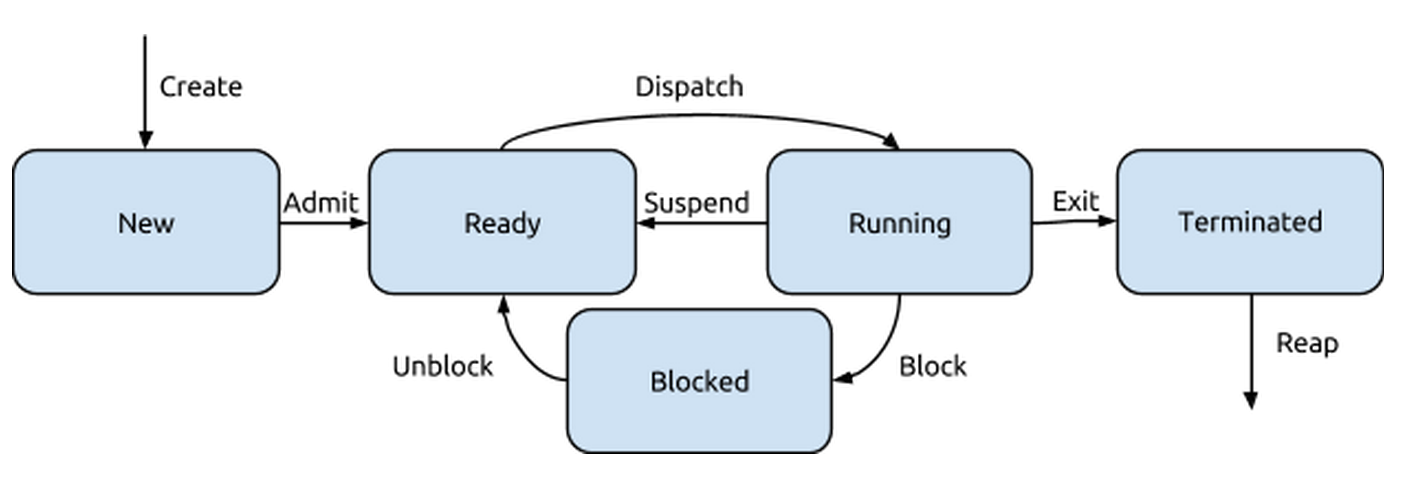
\includegraphics[width=0.9\textwidth]{images/5-state-model.png}
	\end{center}

\end{frame}

\begin{frame}
	\frametitle{Five State Model}

	There are now eight transitions:

	\begin{itemize}
		\item \textbf{Create}
		\item \textbf{Admit}
		\item \textbf{Dispatch}
		\item \textbf{Suspend}
		\item \textbf{Exit}
		\item \textbf{Block}
		\item \textbf{Unblock}
		\item \textbf{Reap}
	\end{itemize}

\end{frame}

\begin{frame}
	\frametitle{Five State Model}

	There are two additional exit transitions that are not shown.

	A process can go directly from ``Ready'' or ``Blocked'' to ``Terminated''.

	This happens if a process is killed.

\end{frame}


\begin{frame}
\frametitle{Threads?}

	Although the concept of the process is important, most operating systems these days think about things at the level of the thread. 

	Almost everything we just learned about process management can apply to thread management!

\end{frame}




\begin{frame}
	\frametitle{What is a Thread?}

	The term ``thread'' is a short form of \alert{Thread of Execution}.

	A thread of execution is a sequence of executable commands that can be scheduled to run on the CPU.

	Threads also have some state and stores some local variables.

	Most programs you will write in other courses have only one thread;\\
	\quad that is, your program's code is executed one statement at a time.

\end{frame}

\begin{frame}
	\frametitle{Multithreaded Programs}

	A multithreaded program uses more than one thread, (some of the time).

	A program begins with an initial thread (where the \texttt{main} method is).

	That main thread can create some additional threads if needed.

	Threads can be created and destroyed within a program dynamically.

\end{frame}

\begin{frame}
	\frametitle{Threads and Processes}

	\begin{center}
		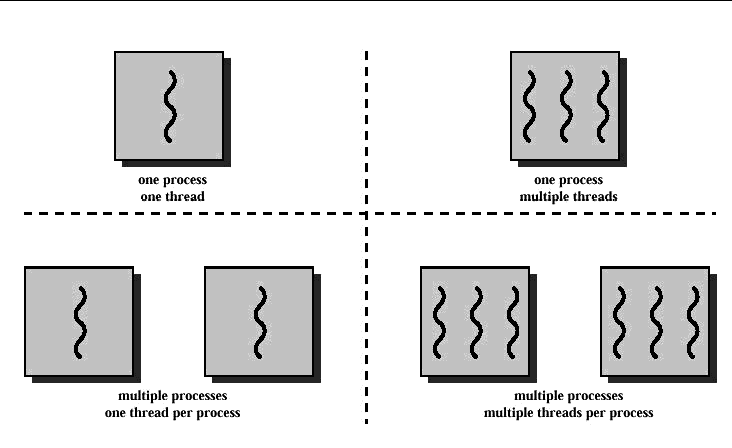
\includegraphics[width=0.9\textwidth]{images/mthread.png}
	\end{center}

\end{frame}

\begin{frame}
	\frametitle{Thread Possessions}


	In a process that has multiple threads, each thread has its own:
	\begin{enumerate}
		\item Thread execution state.
		\item Saved thread context when not running.
		\item Execution stack.
		\item Local variables.
		\item Access to the memory and resources of the process (shared with all threads in that process).
	\end{enumerate}

\end{frame}

\begin{frame}
	\frametitle{Single vs. Multithreaded}

	\begin{center}
		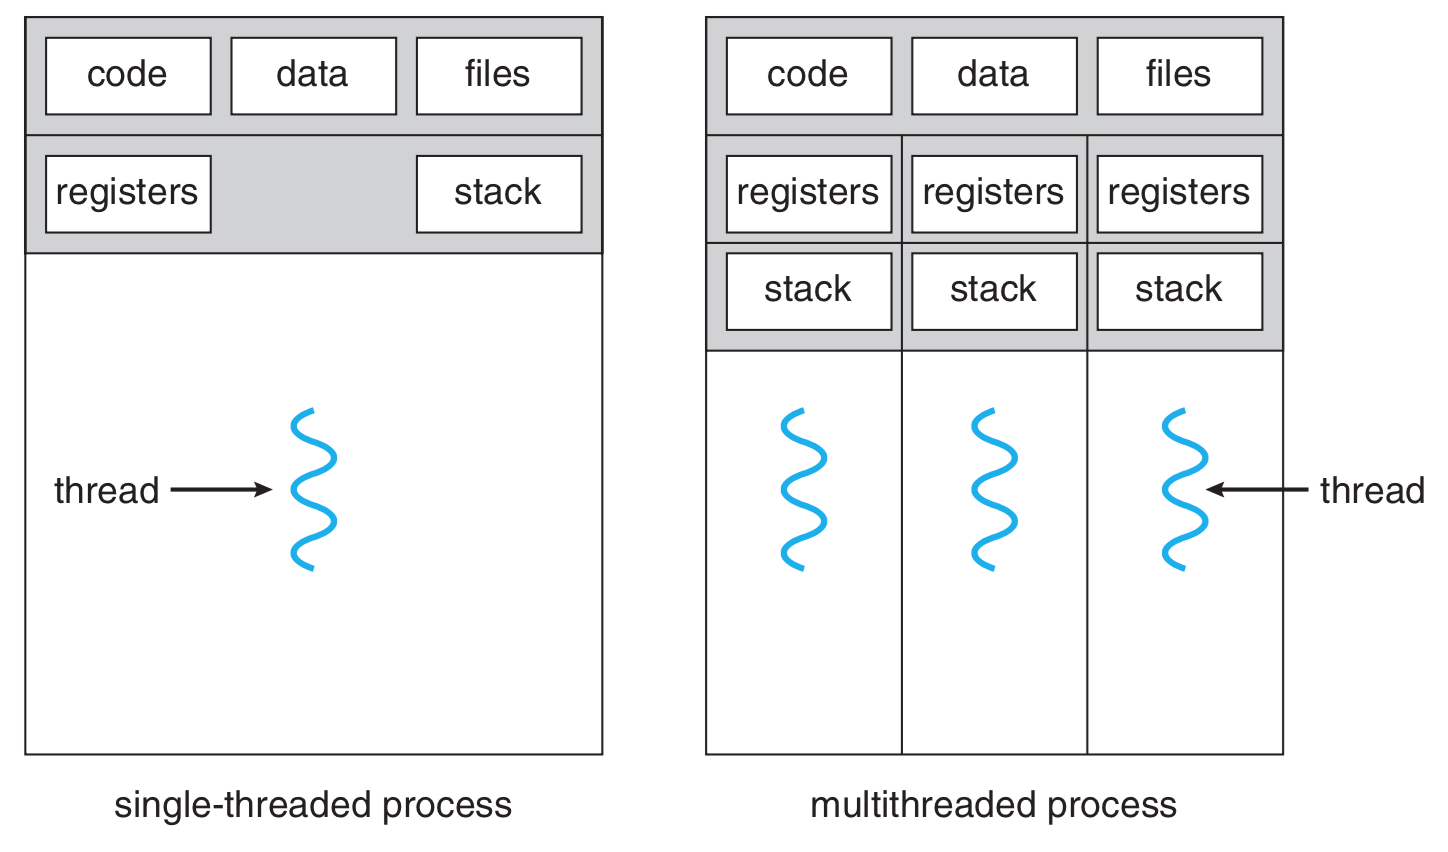
\includegraphics[width=0.9\textwidth]{images/mthread2.png}
	\end{center}

\end{frame}

\begin{frame}
	\frametitle{Thread Notes}

	All the threads of a process share the state and resources of the process.

	If a thread opens a file, other threads in that process can also access it.

	The way programs are written now, few are not multithreaded.



\end{frame}

\begin{frame}
	\frametitle{UI Thread}

	One common way of dividing up the program into threads is to separate the user interface from a time-consuming action.


	File transfer app: If the user interface and upload method share a thread, once a file upload has started, the user will not be able to use the UI anymore.
	
	\begin{center}
	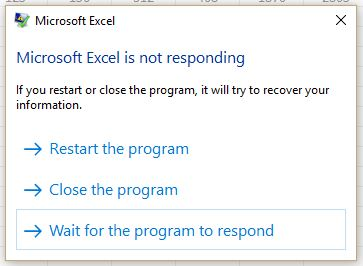
\includegraphics[width=0.4\textwidth]{images/notresponding.png}
	\end{center}

	Not even to click the button that cancels the upload!

\end{frame}

\begin{frame}
	\frametitle{Solving the UI Thread Problem}

	We have two options for how to alleviate this problem.

	Option 1: \texttt{fork} a new process to do the upload; or \\
	Option 2: Spawn  new thread.

	In either case, the newly created entity will handle the upload of the file.

	The UI remains responsive, because the UI thread is not waiting for the upload method to complete.

\end{frame}

\begin{frame}
	\frametitle{Thread Motivation}
	Why threads instead of a new process?

	Primary motivation is: performance.

	\begin{enumerate}
		\item Creation: 10$\times$ faster.
		\item Terminating and cleaning up a thread is faster.
		\item Switch time: 20\% of process switch time.
		\item Shared memory space (no need for IPC).
		\item Lets the UI be responsive.
	\end{enumerate}

\end{frame}

\begin{frame}
	\frametitle{Common Usage of Threads}

	\begin{enumerate}
		\item \textbf{Foreground and Background Work}
		\item \textbf{Asynchronous processing}
		\item \textbf{Speed of Execution}
		\item \textbf{Modular Structure}
	\end{enumerate}

\end{frame}

\begin{frame}
	\frametitle{Thread Drawbacks}

	There is no protection between threads in the same process.

	One thread can easily mess with the memory being used by another.

	This once again brings us to the subject of co-ordination (for later).

	If 1 thread encounters an error, the whole process will be terminated by the OS.

\end{frame}

\begin{frame}
	\frametitle{Thread States}
	Each individual thread will have its own state.
	
	Still using the five state model:

	\begin{center}
		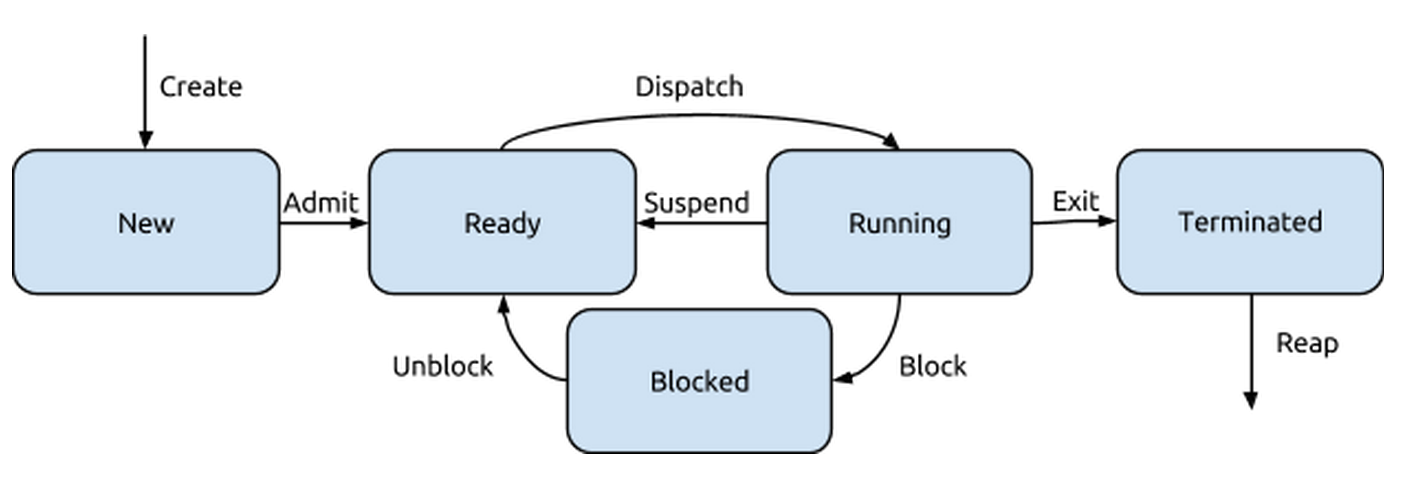
\includegraphics[width=0.85\textwidth]{images/5-state-model.png}
	\end{center}

\end{frame}

\begin{frame}
	\frametitle{Five State Model}

    A thread in any state can transition to terminated.

	When a process is terminated, all its threads are terminated\\
	\quad Regardless of what state it is in.


\end{frame}


\begin{frame}
	\frametitle{Multiprocessing}

	Not that long ago, a typical computer had one processor with one core.

	It could accordingly do exactly one thing at a time.

	1 processor: 1 general purpose processor that executes user processes.

	There may be special-purpose processors in the system (RAID controller).

	Only one general purpose processor so we call it a uniprocessor system.



\end{frame}


\begin{frame}
	\frametitle{Multiprocessing}

	Now, desktops, laptops, and even cell phones are using multi-core processors.

	A quad-core processor may be executing four different instructions from four different threads at the same time.

	In theory, multiple processors may mean that we can get more work done in the same amount of (wall clock) time, but this is not a guarantee.

\end{frame}


\begin{frame}
	\frametitle{Terminology Note}


	Terminology note: we often refer to a logical processing unit as a \alert{core}.

	CPU may refer to a physical chip that contains 1+ logical processing units.

	As far as the operating system is concerned, it does not much matter if a system has four cores in four physical chips or four cores in one chip.

	Either way, there are four units that can execute instructions.



\end{frame}


\begin{frame}
	\frametitle{Execution}

	1 process, 1 thread: it does not matter how many cores are available.\\
	\quad At most one core will be used to execute this task.

	If there are multiple processes, each process can execute on a different core.

	But what if there are more processes and threads than available cores?

	We can hope that the processes get blocked frequently enough and long enough?



\end{frame}


\begin{frame}
	\frametitle{Chest Day Best Day}

	\begin{center}
		
\includegraphics[width=0.5\textwidth]{images/chestdaybestday.png}
	\end{center}

	``Can I work in with you?''

\end{frame}


\begin{frame}
	\frametitle{Execution}


	Switch between the different tasks via a procedure we call \alert{time slicing}.

	So thread 1 would execute for a designated period, such as 20 ms, then thread 2 for 20 ms, then thread 3 for 20 ms, then back to thread 1 for 20 ms.

	To the user, it seems like threads 1, 2, and 3 are being executed in parallel.\\
	\quad 20 ms is fast enough that the user does not notice the difference.

\end{frame}


\begin{frame}
	\frametitle{Single Core Execution}

	\begin{center}
		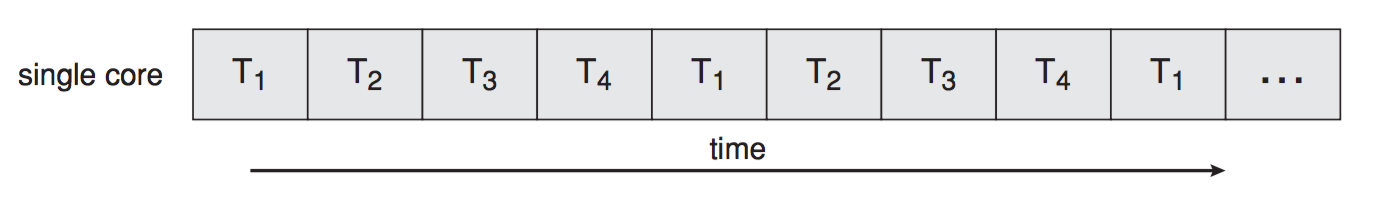
\includegraphics[width=\textwidth]{images/single-core-execution.png}
	\end{center}

\end{frame}


\begin{frame}
	\frametitle{Multi Core Execution}

	Time slicing will still occur, if necessary:

	\begin{center}
		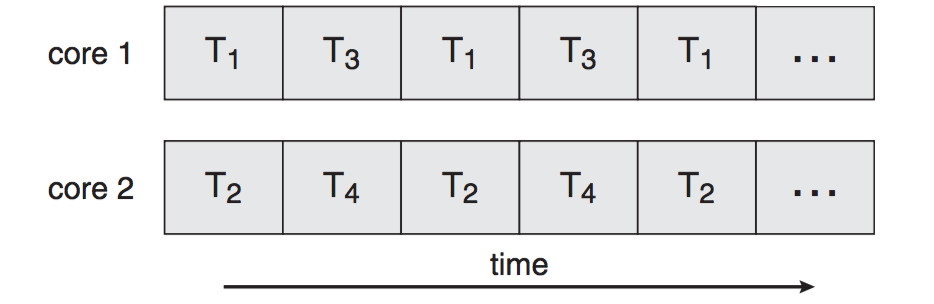
\includegraphics[width=\textwidth]{images/dual-core-execution.png}
	\end{center}


\end{frame}



\begin{frame}
	\frametitle{Parallelism}

	Multiple threads at the same time = tasks completed faster?

\end{frame}

\begin{frame}
	\frametitle{Parallelism and Speedup}

	Depends on the nature of the task!

	Fully parallelized: 2 $\times$ Threads = 2 $\times$ Speed

	Partially parallelized: 2 $\times$ Threads = $(1 < n < 2)$ $\times$ Speed

	Cannot be parallelized: 2 $\times$ Threads = $1$ $\times$ Speed

\end{frame}


\begin{frame}
	\frametitle{Heard, Chef!}

	\begin{center}
		
\includegraphics[width=\textwidth]{images/lamb-sauce.jpg}
	\end{center}

\end{frame}



\begin{frame}
	\frametitle{Speedup Example}


	Suppose: a task that can be executed in 5~s, containing a parallelizable loop.

	Initialization and recombination code in this routine requires 400~ms.

	So with one processor executing, it would take about 4.6~s to execute the loop.

	Split it up and execute on two processors: about 2.3~s to execute the loop.

	Add to that the setup and cleanup time of 0.4~s and we get a total time of 2.7~s.

	Completing the task in 2.7~s rather than 5~s represents a speedup of about~46\%.

\end{frame}


\begin{frame}
	\frametitle{Amdahl's Law}

	Gene Amdahl came up with a formula for the general case of how much faster a task can be completed based on how many processors we have available.

	Let us define $S$ as the portion of the application that must be performed serially and $N$ as the number of processing cores available.

	Amdahl's Law:

	\begin{center}
		speedup $\leq$ {\huge $\frac{1}{S + \frac{1-S}{N}}$}
	\end{center}

\end{frame}


\begin{frame}
	\frametitle{Amdahl's Law}

	Take the limit as $N \rightarrow$ infinity and you will find the speedup converges to $\frac{1}{S}$.


	The limiting factor on how much additional processors help is the size of $S$.

	Matches our intuition of how it should work.

\end{frame}


\begin{frame}
	\frametitle{Amdahl's Law on the 5~s Task}

	Applying this formula to the example from earlier:

	\begin{center}
		\begin{tabular}{l|l}
			\textbf{Processors} & \textbf{Run Time (s)} \\ \hline
			1                   & 5                     \\
			2                   & 2.7                   \\
			4                   & 1.55                  \\
			8                   & 0.975                 \\
			16                  & 0.6875                \\
			32                  & 0.54375               \\
			64                  & 0.471875              \\
			128                 & 0.4359375             \\
		\end{tabular}
	\end{center}

\end{frame}


\begin{frame}
	\frametitle{Observations on the 5~s Task}

	1. Diminishing returns as we add more processors.

	2. Converges on 0.4~s.

	The most we could speed up this code is by a factor of $\frac{5}{0.4}\approx 12.5$.

	But that would require infinite processors (and therefore infinite money).

\end{frame}


\begin{frame}
	\frametitle{Merge Sort Example}

	Recall from data structures and algorithms the concept of merge sort.

	This is a divide-and-conquer algorithm like binary search.

	Split the array of values up into smaller pieces, sort those, and then merge the smaller pieces together to have sorted data.


\end{frame}


\begin{frame}
	\frametitle{Merge Sort Example}

	\begin{center}
		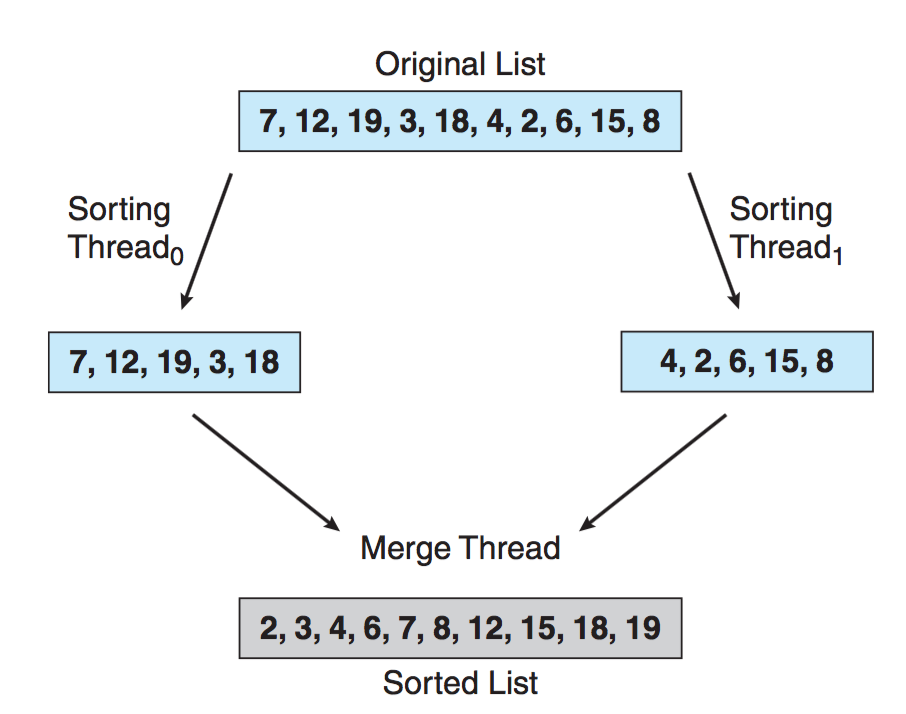
\includegraphics[width=0.75\textwidth]{images/multithread-sort.png}
	\end{center}


\end{frame}



\end{document}

